The SBND is another LArTPC detector part of the Short-Baseline Neutrino Program, together with MicroBooNE and ICARUS-T$600$. It is currently under construction and will consist of a $112$-ton LArTPC located at the BNB beamline. The diagram view of the SBN program detectors and their respective positions in the BNB beamline is shown in figure \ref{fig:sbn}.

\begin{figure}[h!]
    \centering
    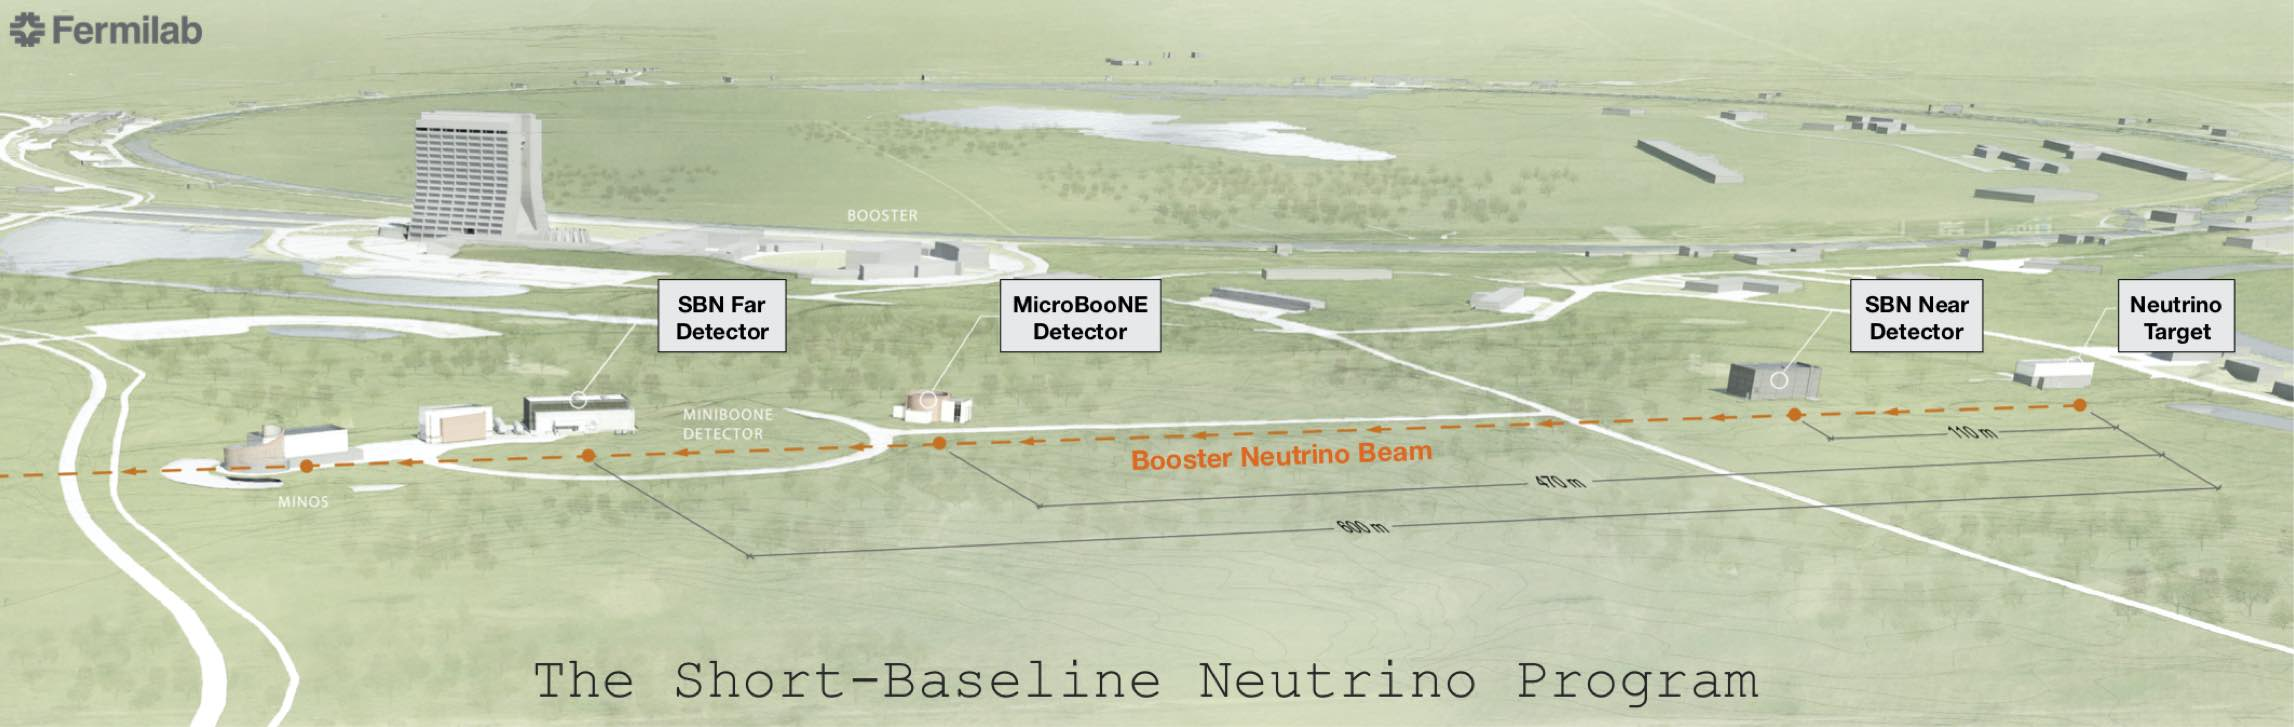
\includegraphics[width=115mm]{Figures/sbn.jpg}
    \caption{Diagram view of the SBN program at Fermilab \cite{SBN}.}
    \label{fig:sbn}
\end{figure}

This LArTPC in particular is made of two different drift regions of $2$ m, with a central cathode, and two wire readout planes. A diagram of SBND and pictures of its anode planes are shown in picture \ref{fig:sbnd}. 

\begin{figure}[h!]
    \centering
    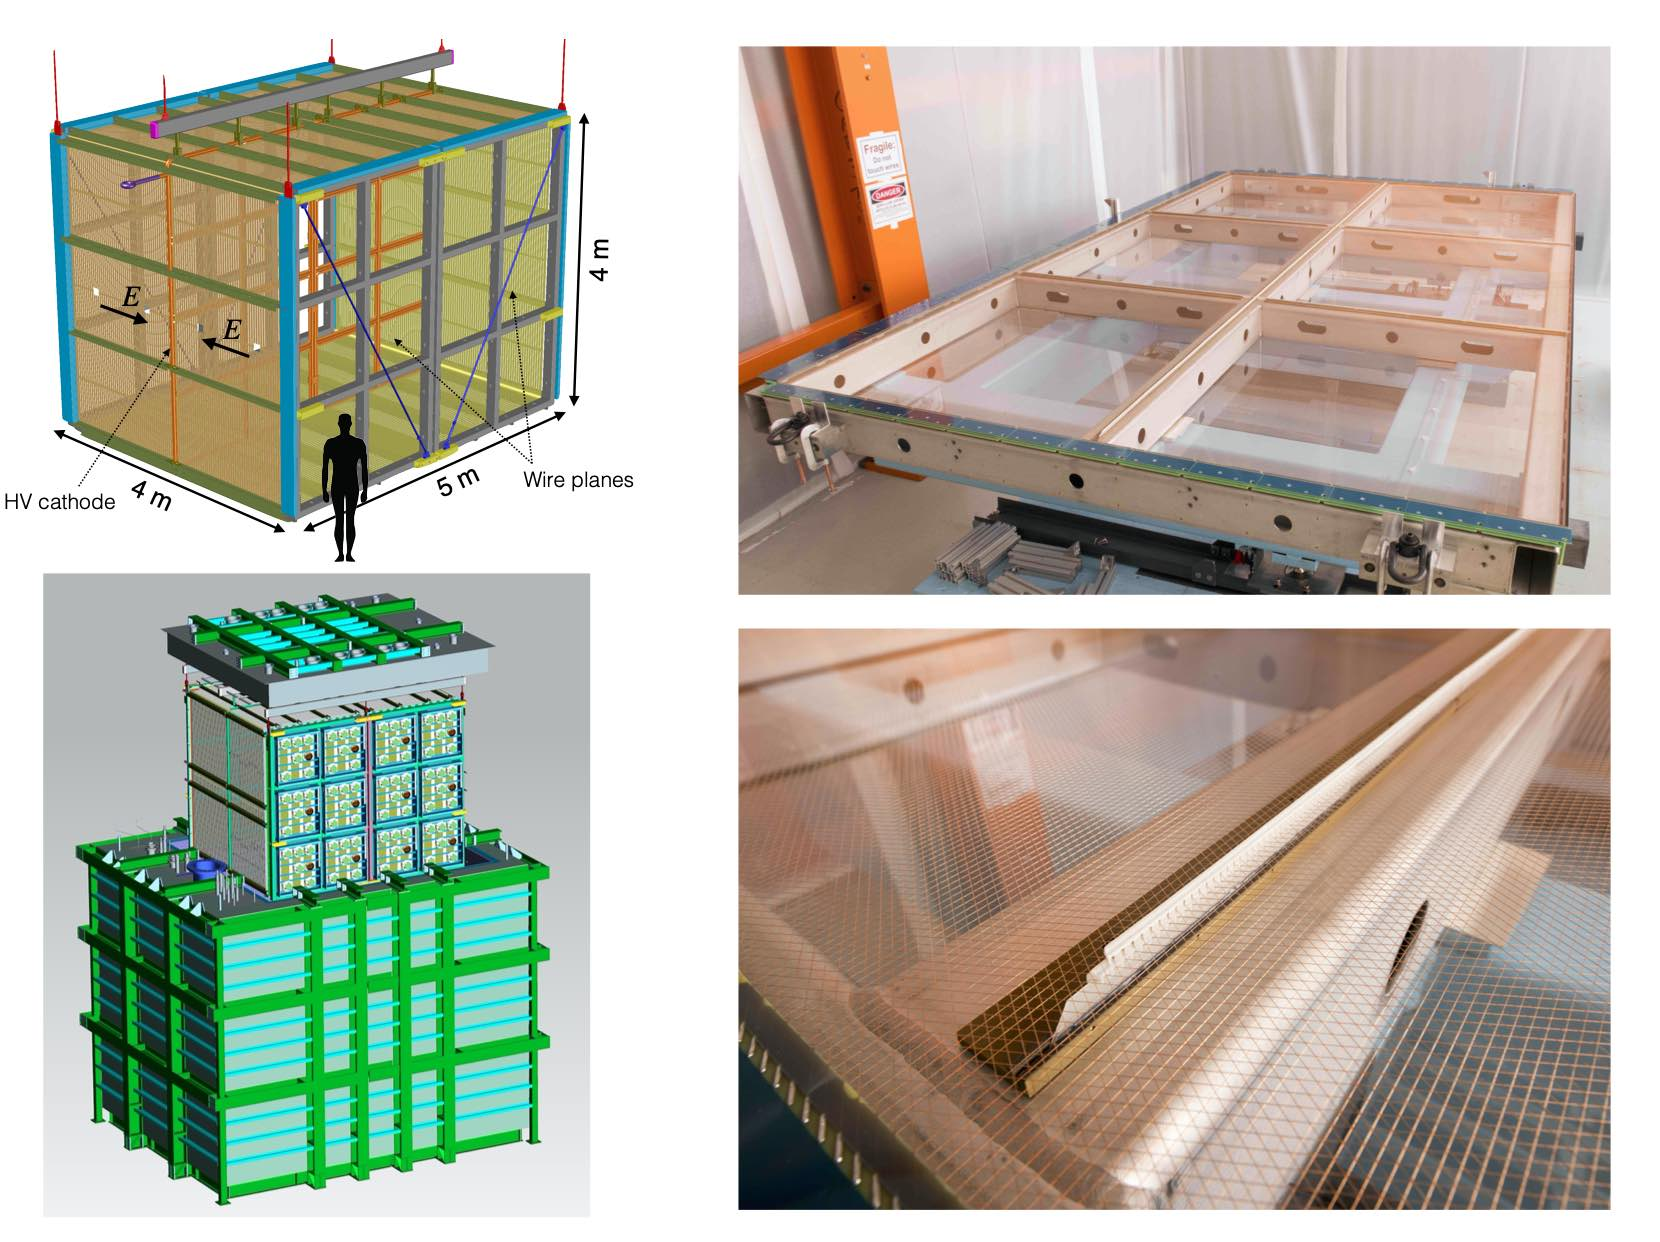
\includegraphics[width=110mm]{Figures/sbnd.jpg}
    \caption{Diagram view of the SBND detector on the left and pictures of SBND's anode wire planes on the right \cite{SBN}.}
    \label{fig:sbnd}
\end{figure}

The frame structures that you can see in the top left of figure \ref{fig:sbnd} are called Anode Plane Assemblies (APA). SBND has two of these frames. For each of them, half of the structure was made by our group and the other half was made by the Manchester group. We have a total of four structures, two made by our group and two made by the Manchester group, that in the end  form two APAs, one that is placed at the West side and another at the East side of the detector. 

\section{TPC Assembly and Installation}

After unboxing the APA structures, other members of the SBND assembly crew and I moved each of them to a clean tent where there is an alignment table. You can see the pictures of the tent and the APAs placed on the alignment table on picture \ref{fig:eastAPA}.

\begin{figure}[ht!]
    \centering
    \begin{subfigure}[t]{0.5\textwidth}
        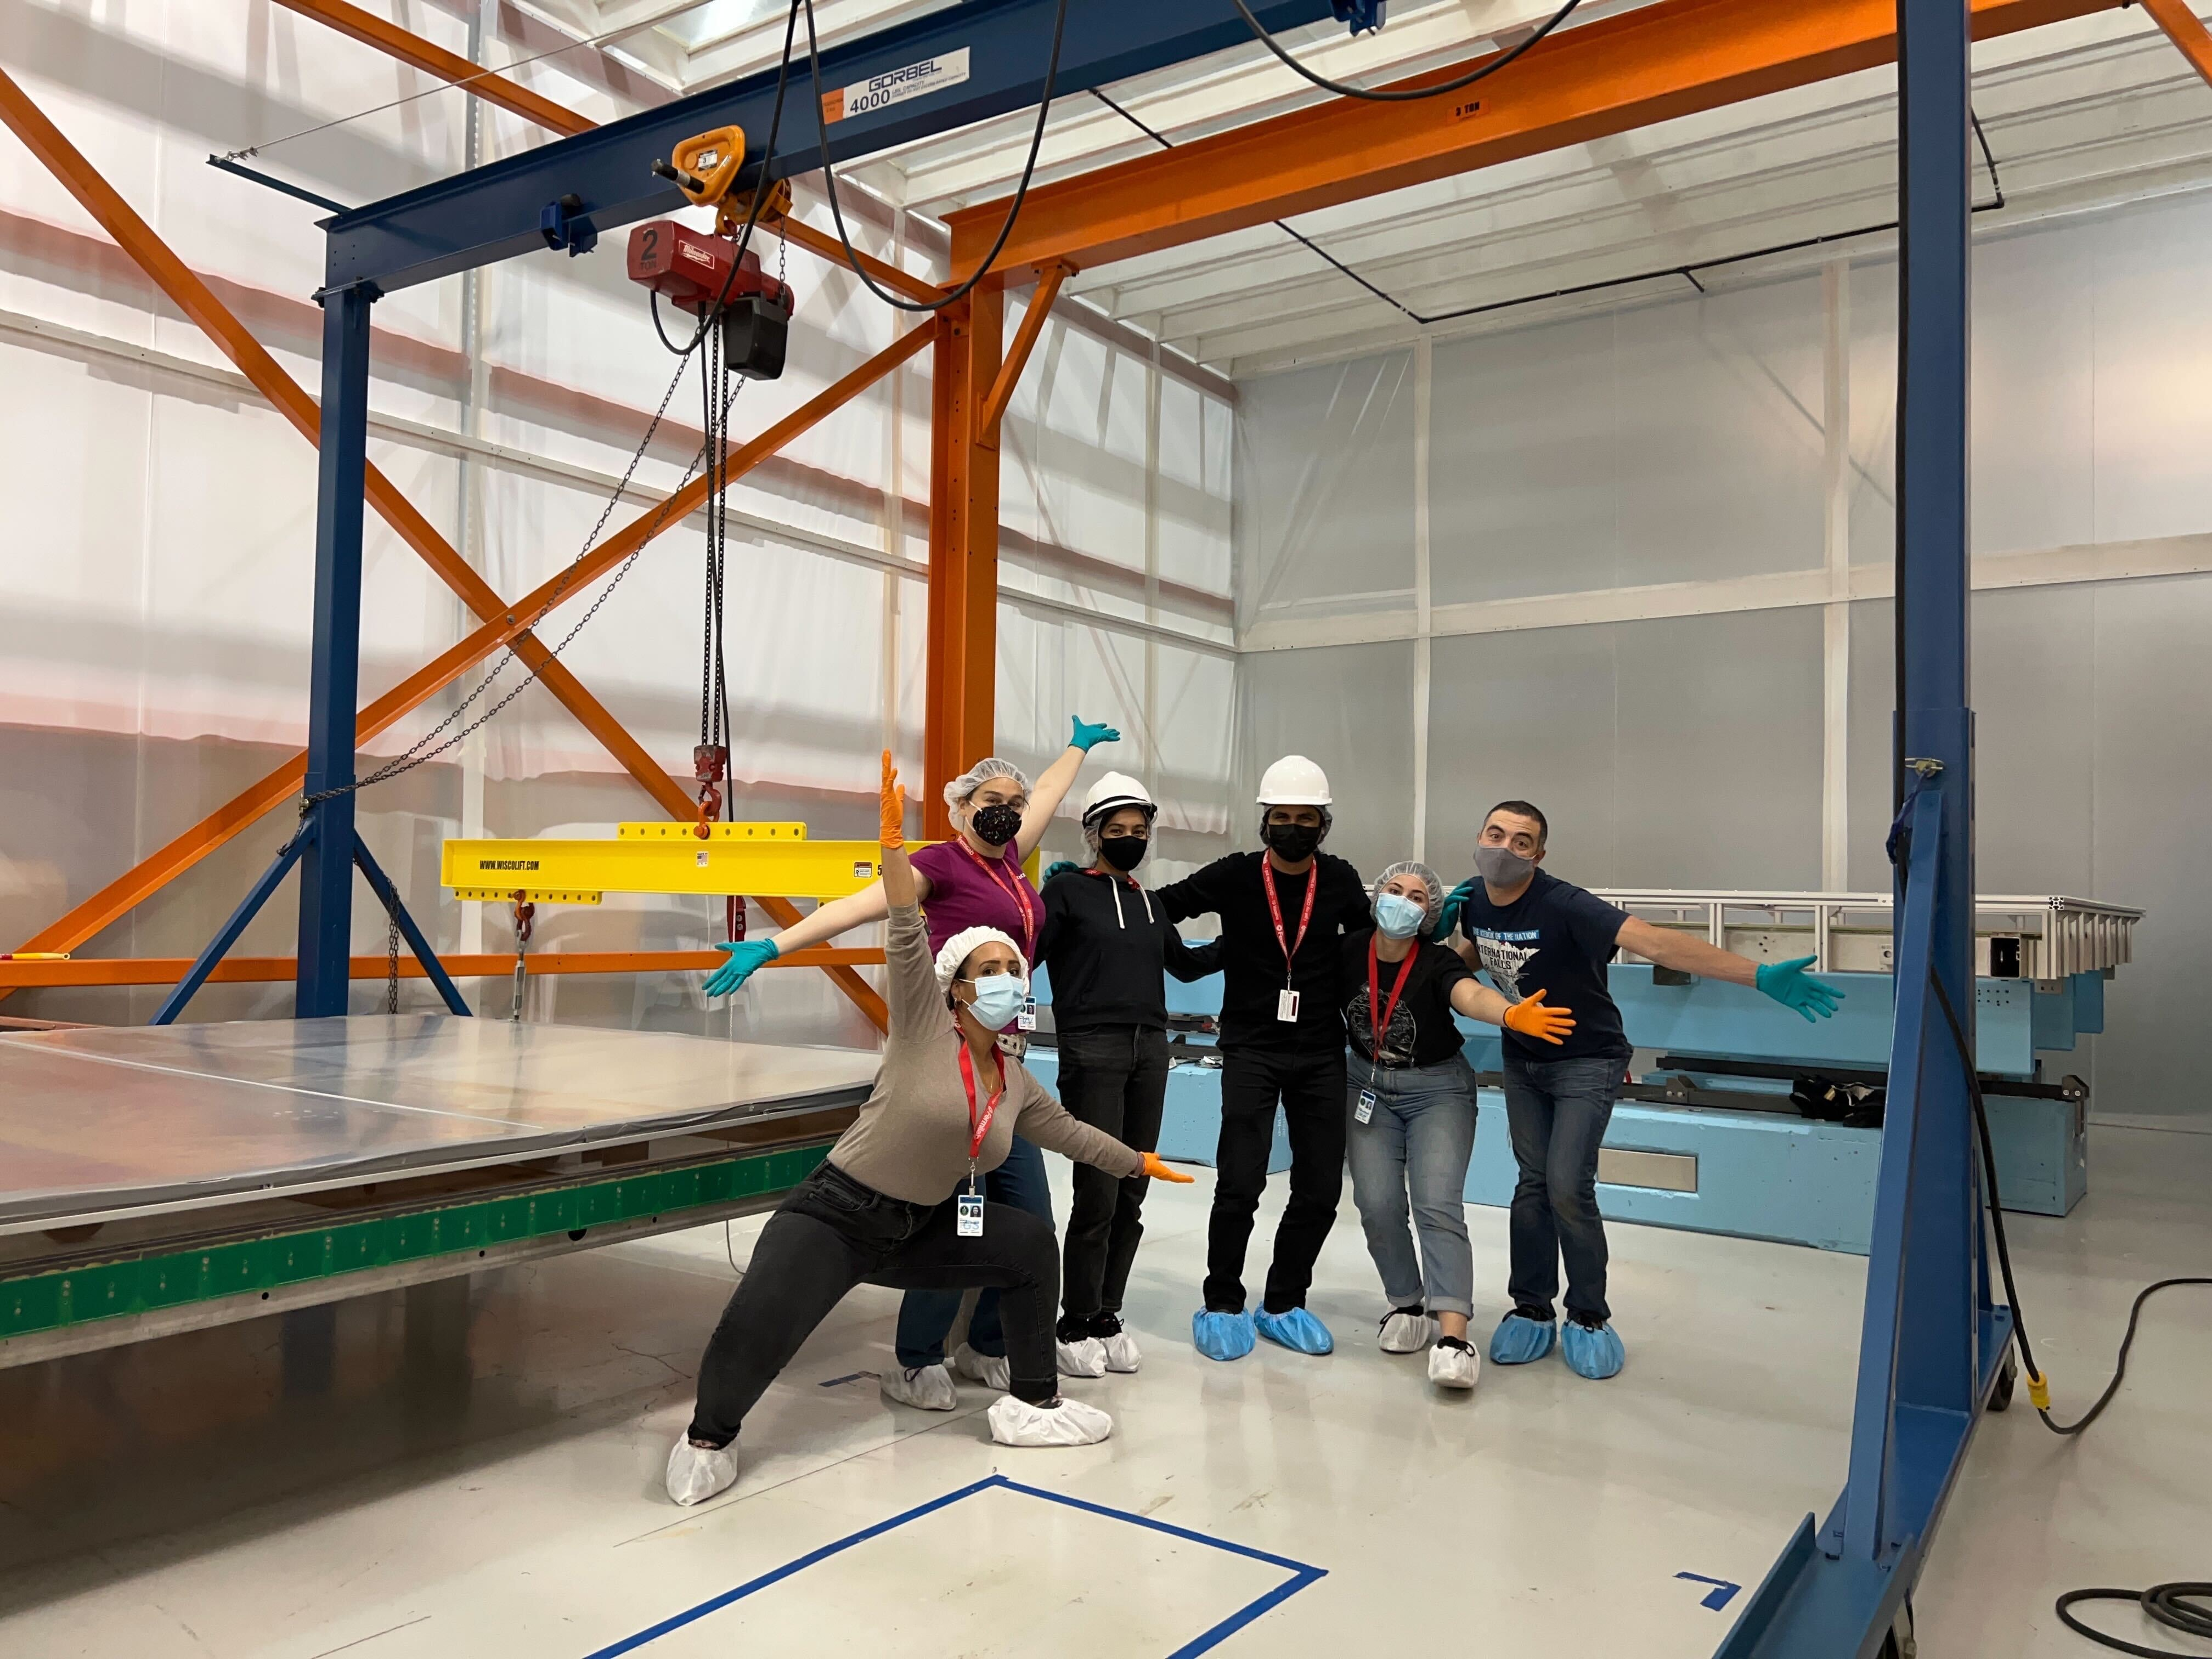
\includegraphics[width=\textwidth]{Figures/eastAPA_post.jpg}
        \caption{}
    \end{subfigure}
    \hfill
    \begin{subfigure}[t]{0.49\textwidth}
        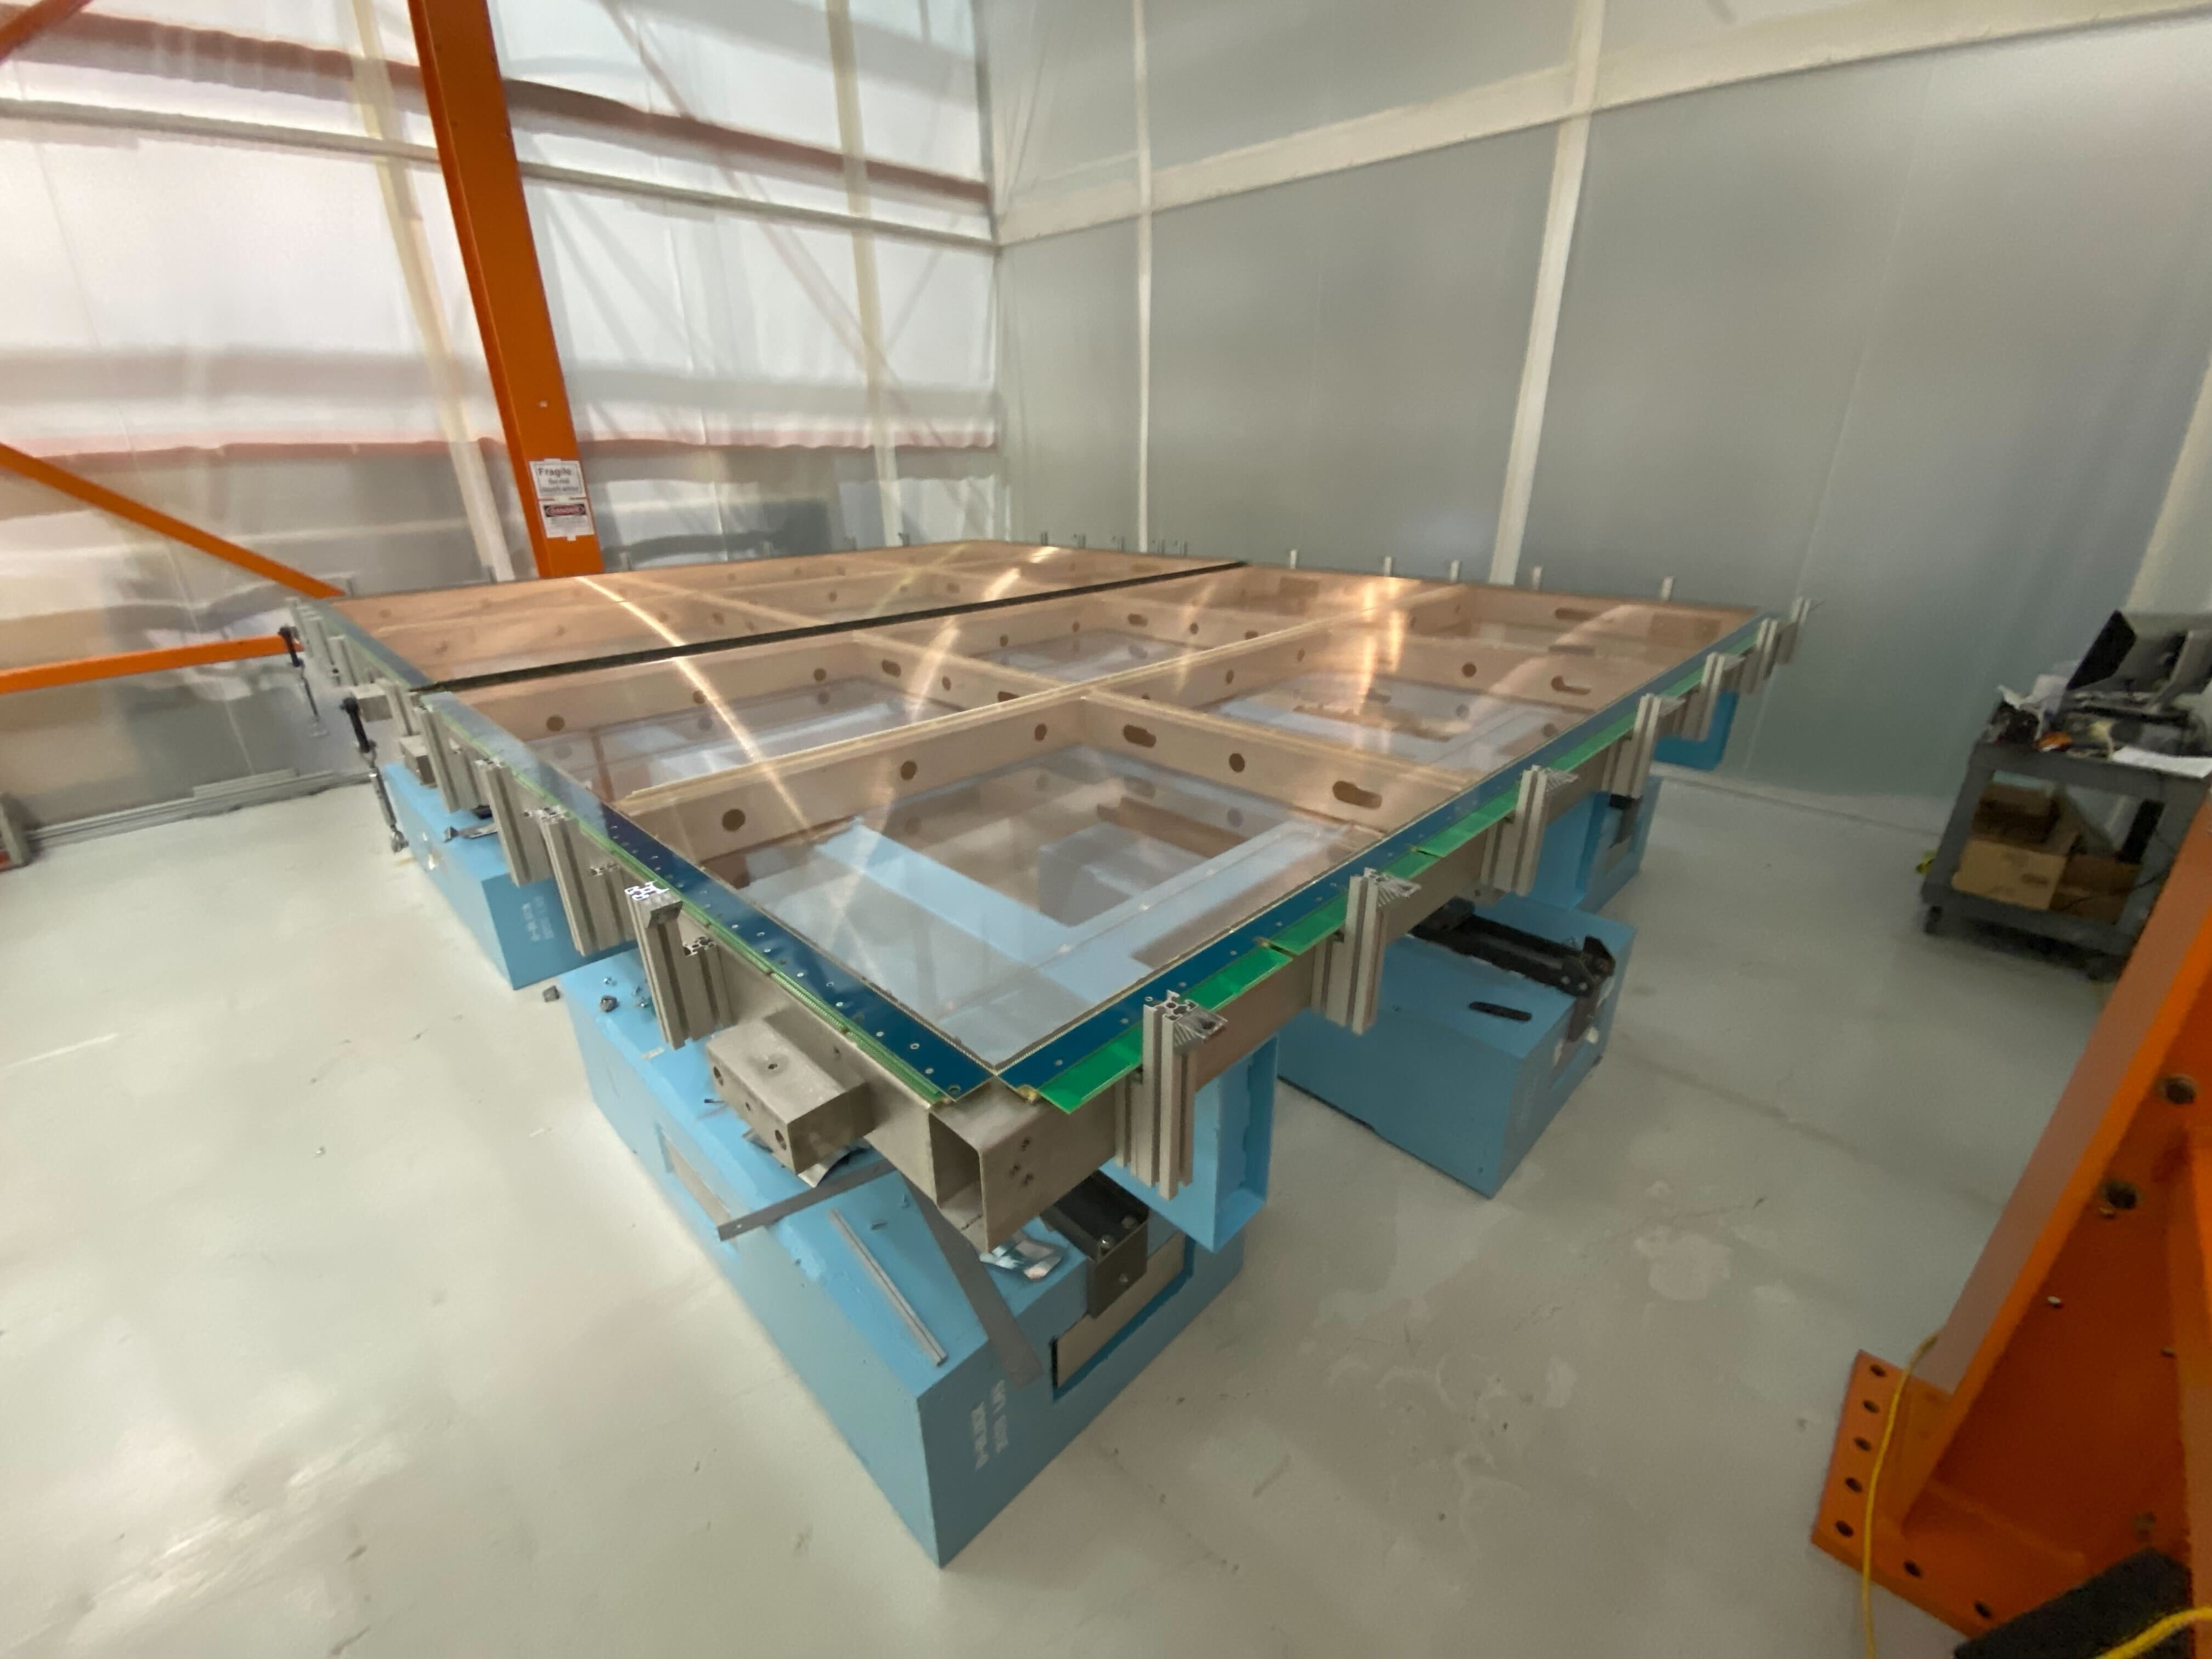
\includegraphics[width=\textwidth]{Figures/east_APA_pre.jpg}
        \caption{}
    \end{subfigure}
    \caption{On the left, a picture of the on-site crew that were working on moving the East APA to the alignment table. In it, you can see a half of an APA resting on the crib before its placement on the alignment table. On the right, a half of an APA recently placed on the alignment table.}
    \label{fig:eastAPA}
\end{figure}

 We then placed the two halves of the APA (one assembled by the SU team and another by the Manchester team) at each side of the table. We tested if the wires kept their nominal mechanical tensions and are still electrically conducting. Next, we aligned each frame and attached them, both mechanically and electrically, to form one bigger APA structure. On picture \ref{fig:aligment} you can see us working with Fermilab's alignment team on the East APA alignment. 

 \begin{figure}[h!]
    \centering
    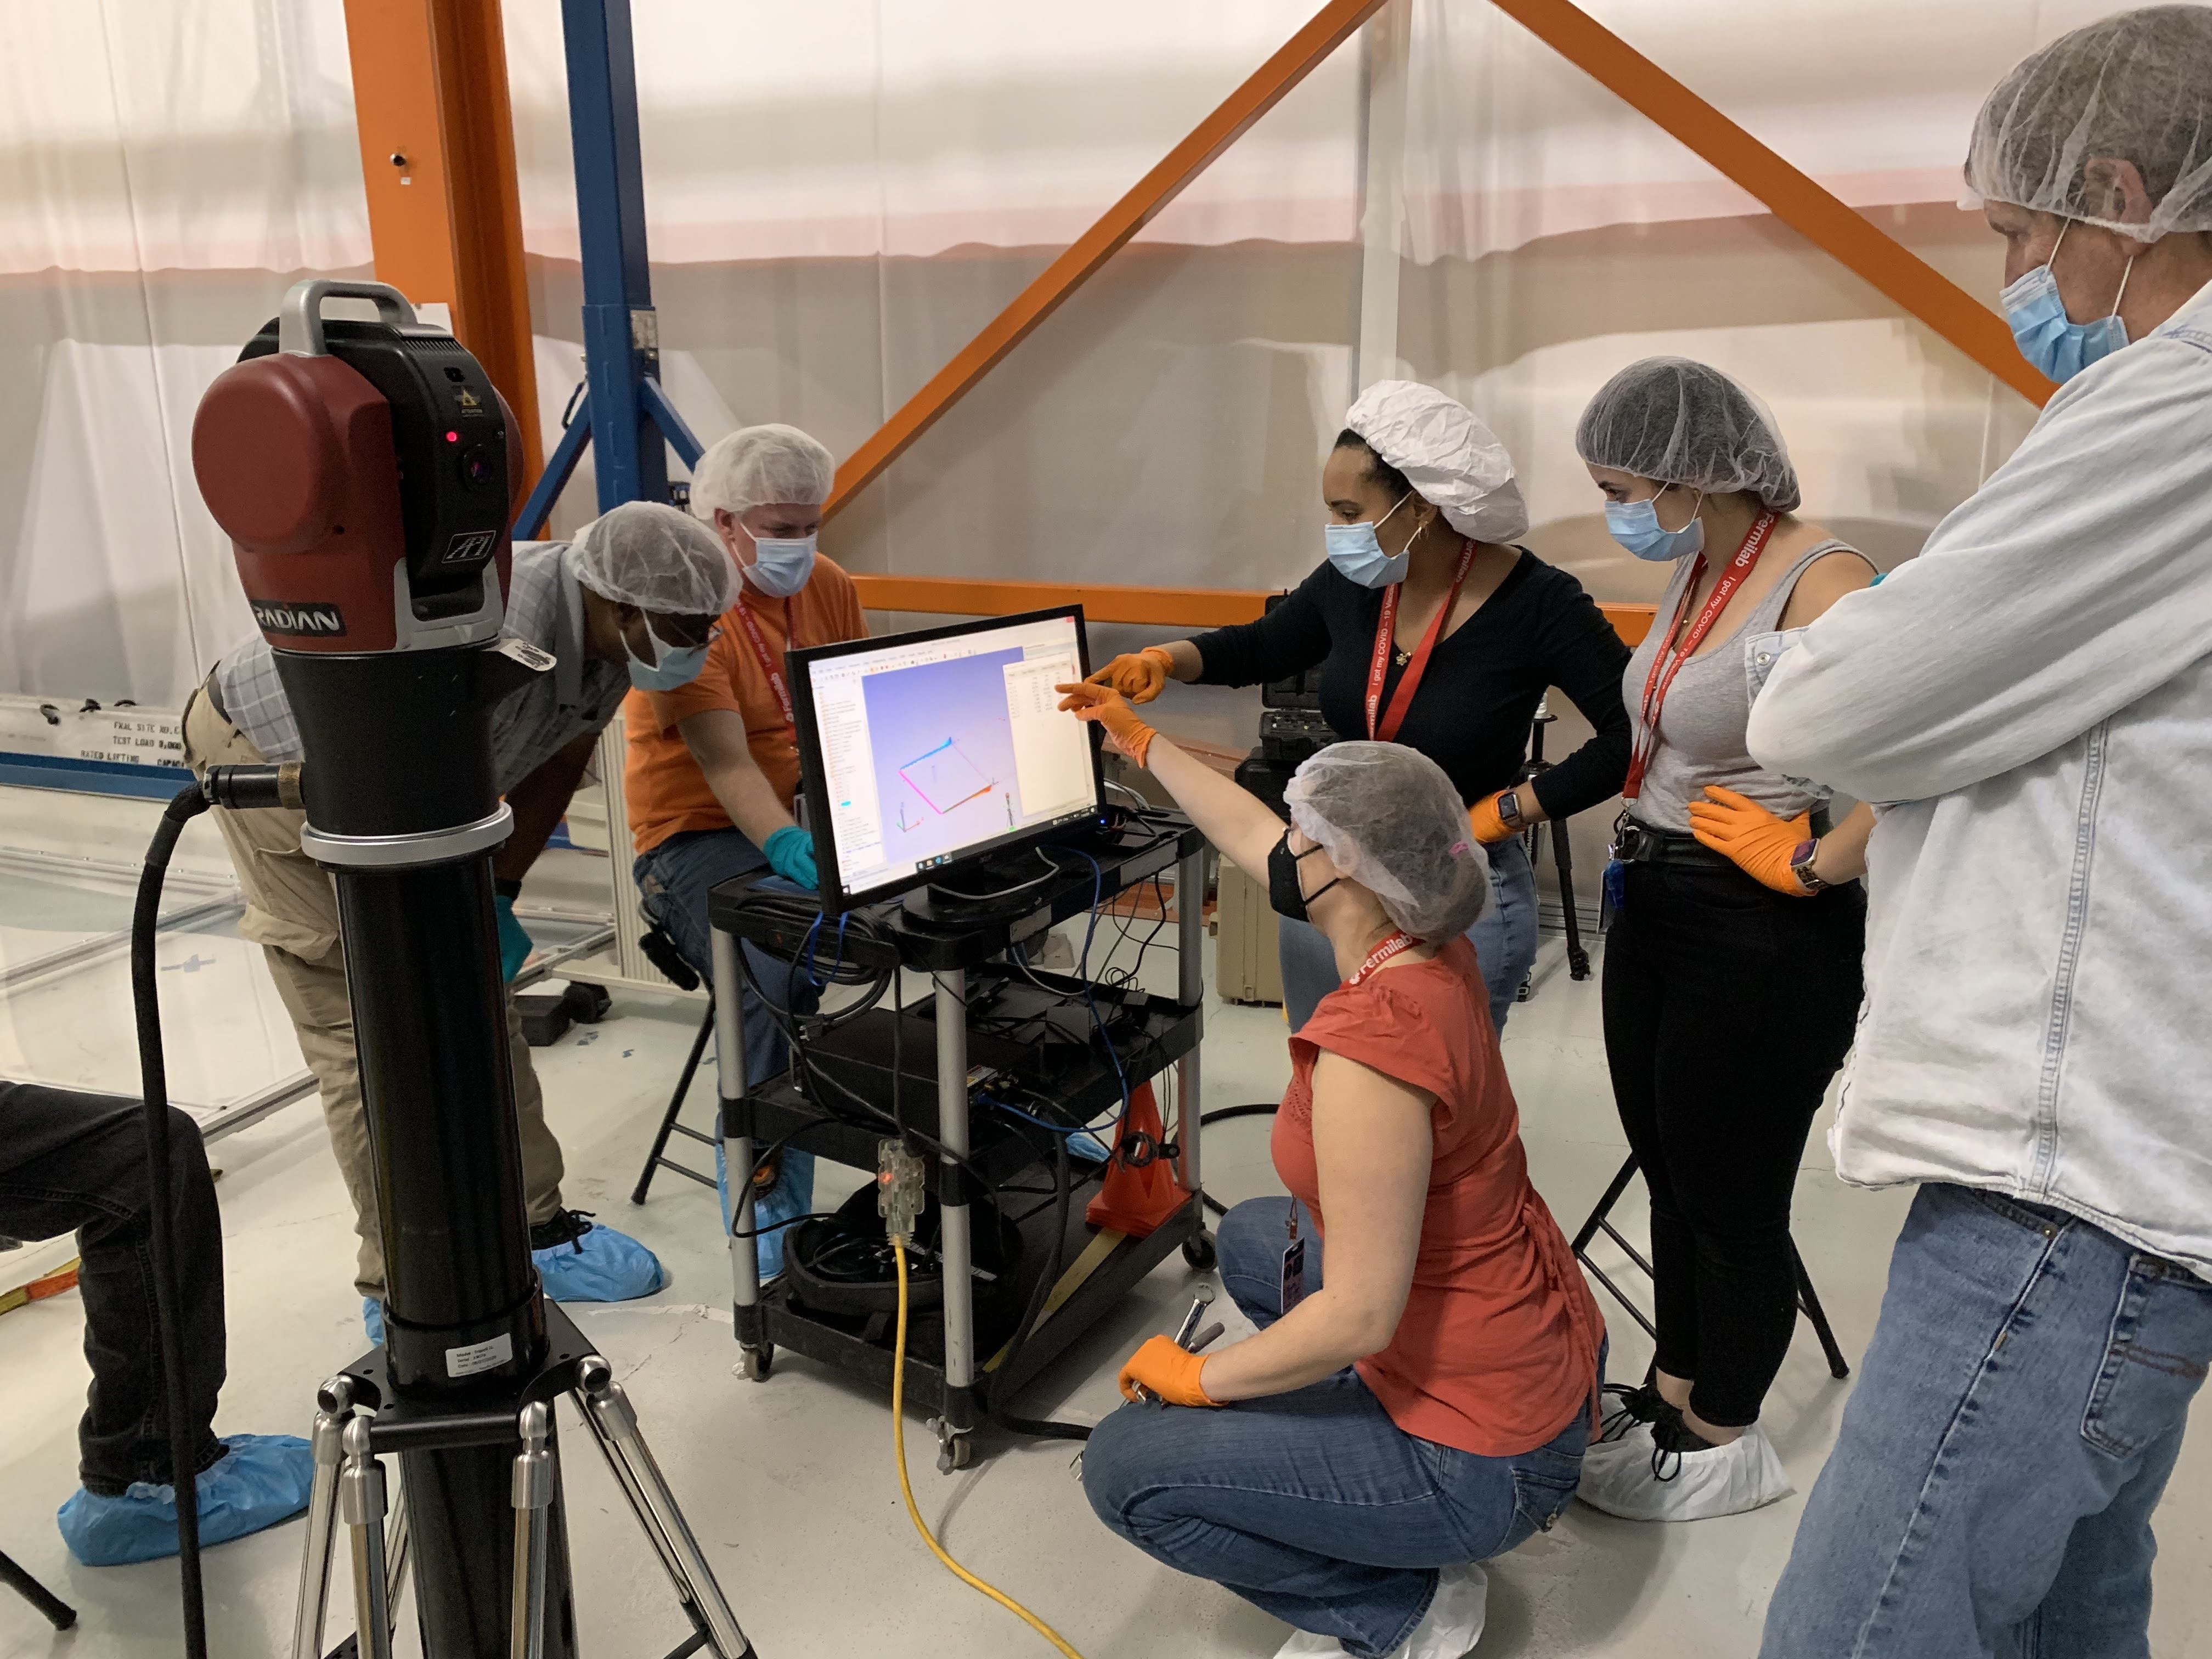
\includegraphics[width=80mm]{Figures/IMG_3794.jpeg}
    \caption{SBND's team working with Fermilab's alignment team on the East APA alignment.}
    \label{fig:aligment}
\end{figure}

Next, the APA is carefully taken from the clean tent where we performed all the tests and placed in still final place in an structure called the Assembly Transport Frame (ATF), that supports the individual components of the TPC in place. We repeated all the procedures for the West APA.
\begin{figure}[ht!]
    \centering
    \begin{subfigure}[t]{0.46\textwidth}
        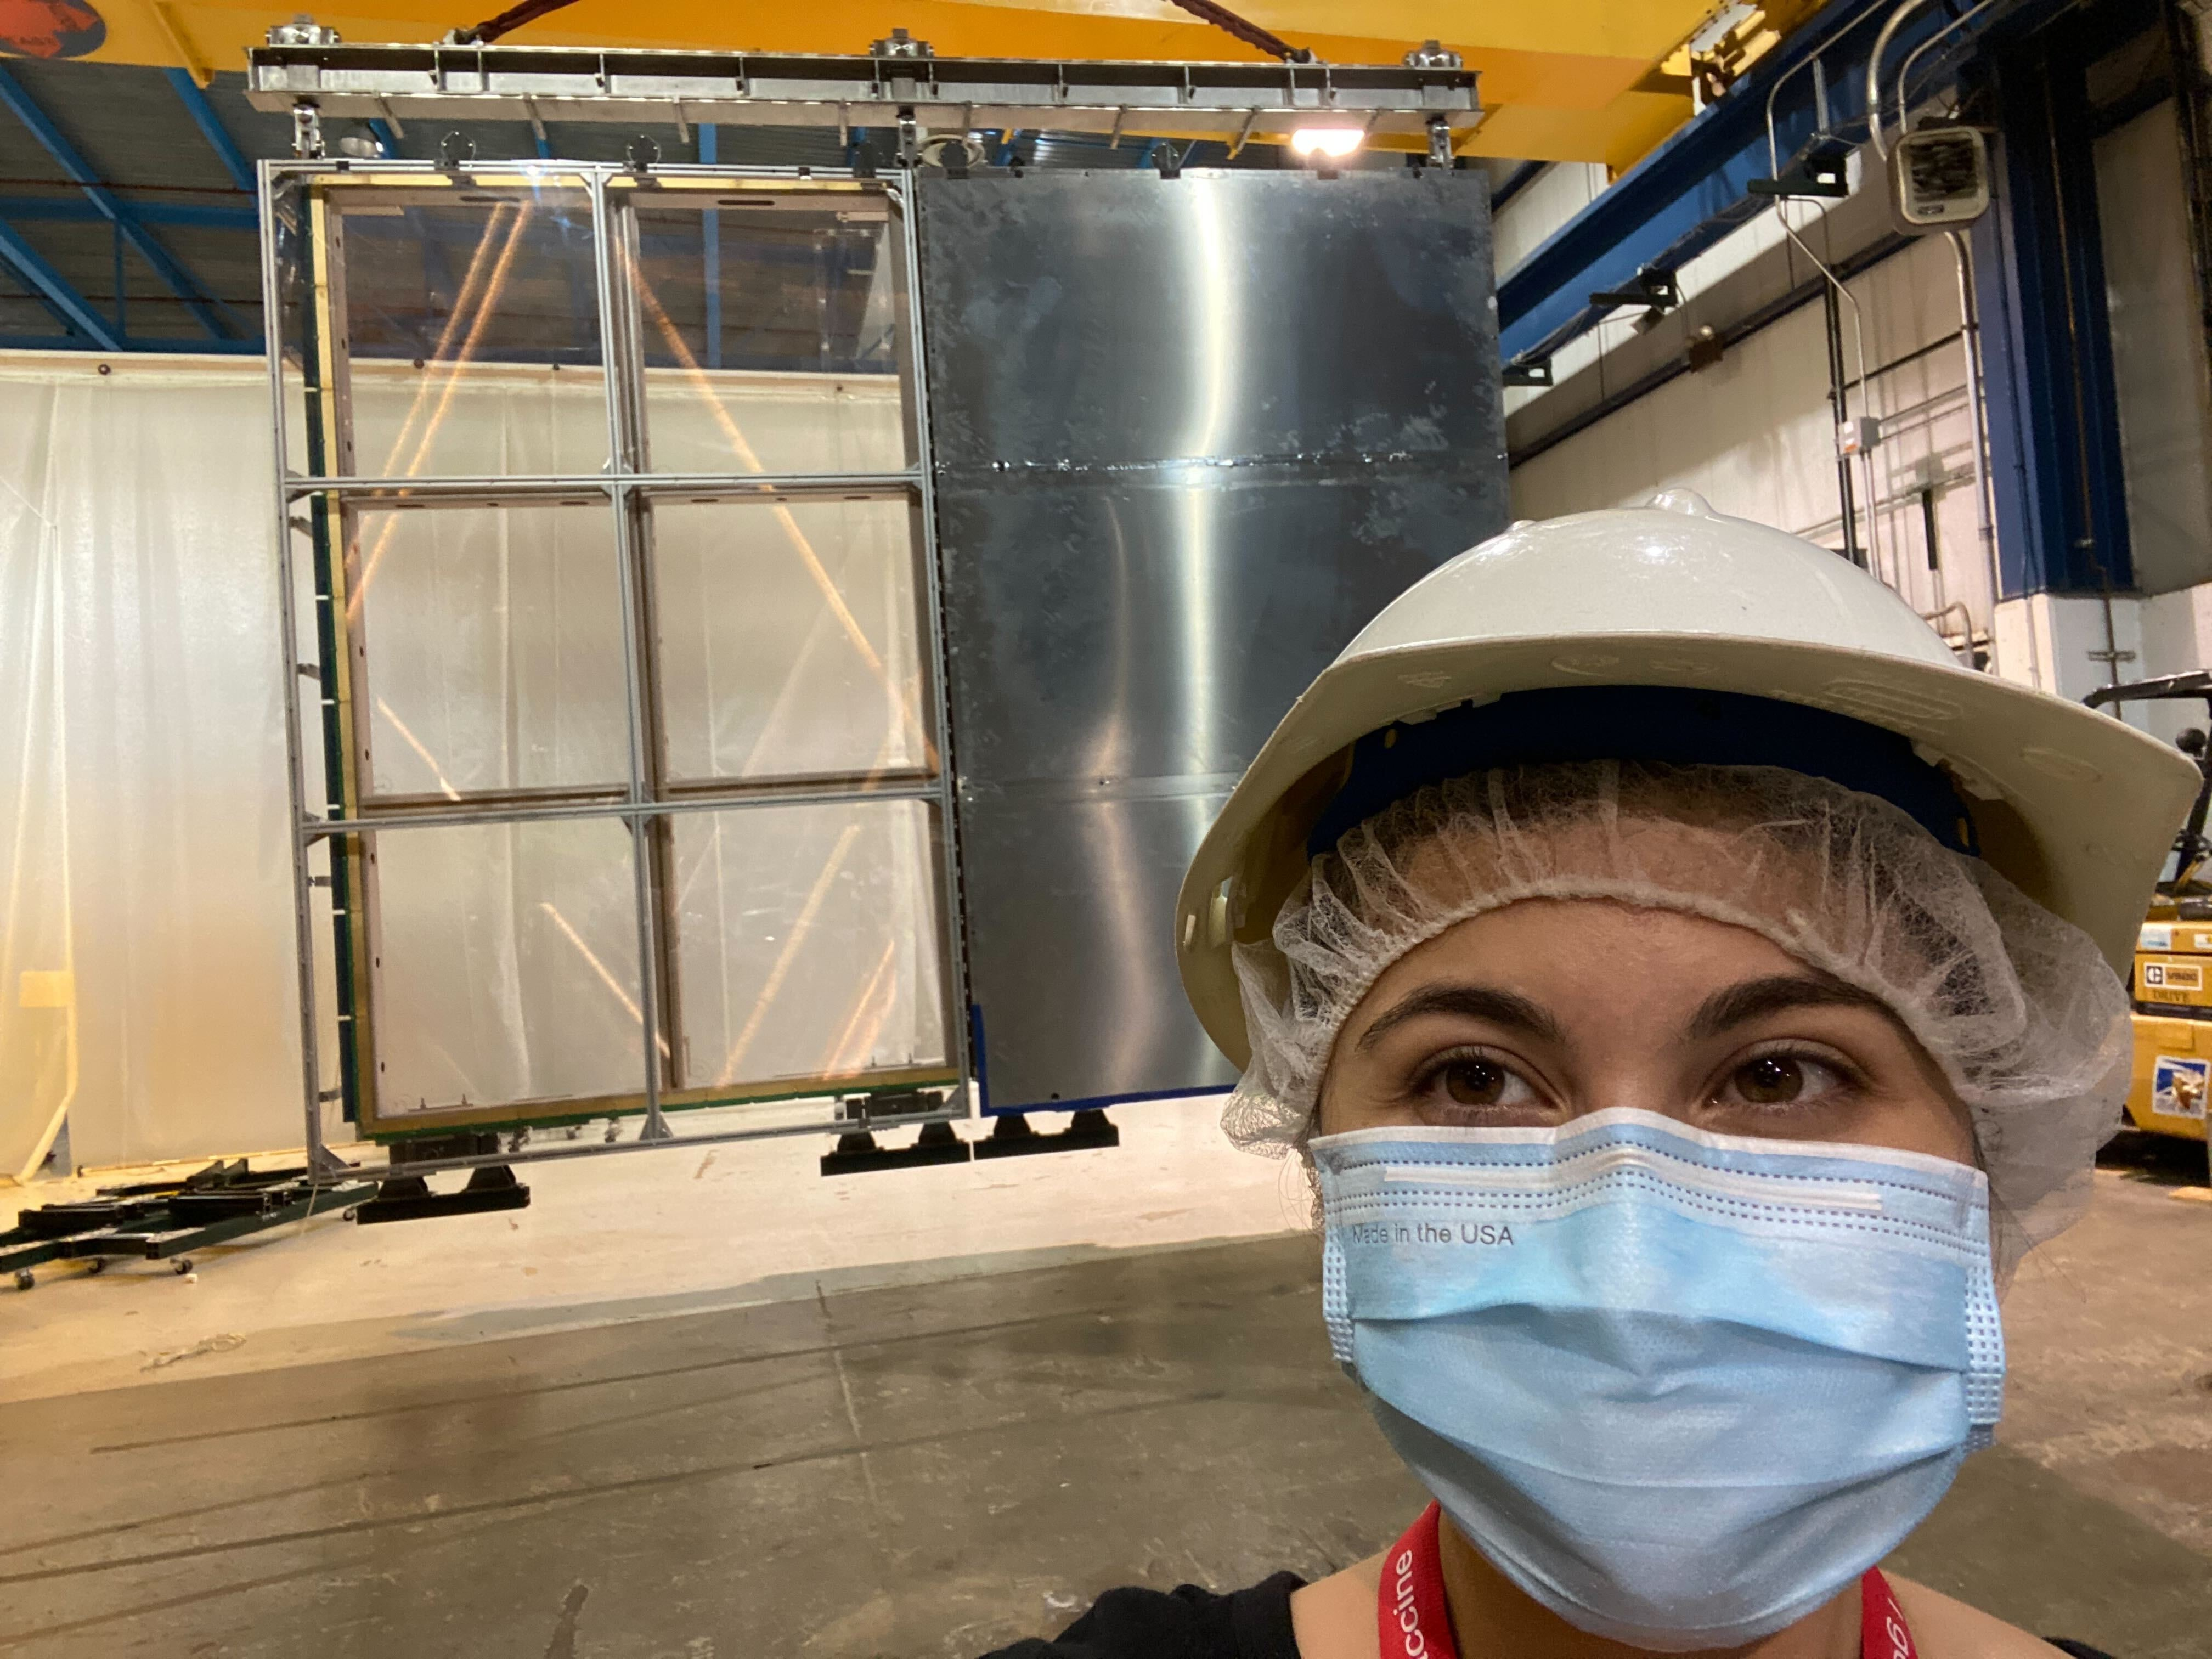
\includegraphics[width=\textwidth]{Figures/west_APA_pre.jpg}
        \caption{}
    \end{subfigure}
    \hfill
    \begin{subfigure}[t]{0.49\textwidth}
        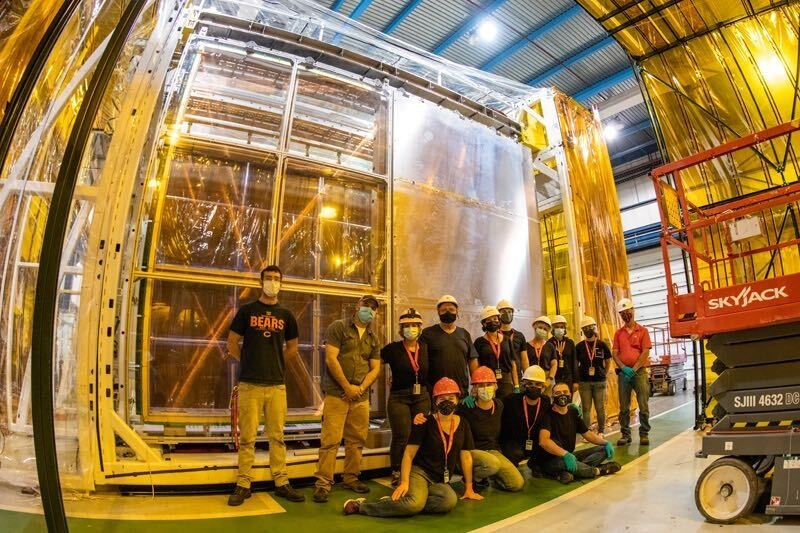
\includegraphics[width=\textwidth]{Figures/westAPA_post.jpg}
        \caption{}
    \end{subfigure}
    \caption{On the left, a picture of me during and the West APA during the moving to its final place in the TPC. You can see the APA frame hanging by the crane during the operation. On the right, the on-site crew in front of the newly-installed West APA in the TPC.}
    \label{fig:westAPA}
\end{figure}

After both APAs were installed in the ATF and aligment adjusted, we started the field cage installation. The field cage are metal structures responsible to guarantee the shape and the uniformity of the electric field. In SBND, we have 8 field cage modules in each side of the detector, bottom, top, North, and South. You can see some pictures of the field cage installation in \ref{field_cage}

\begin{figure}[ht!]
    \centering
    \begin{subfigure}[t]{0.48\textwidth}
        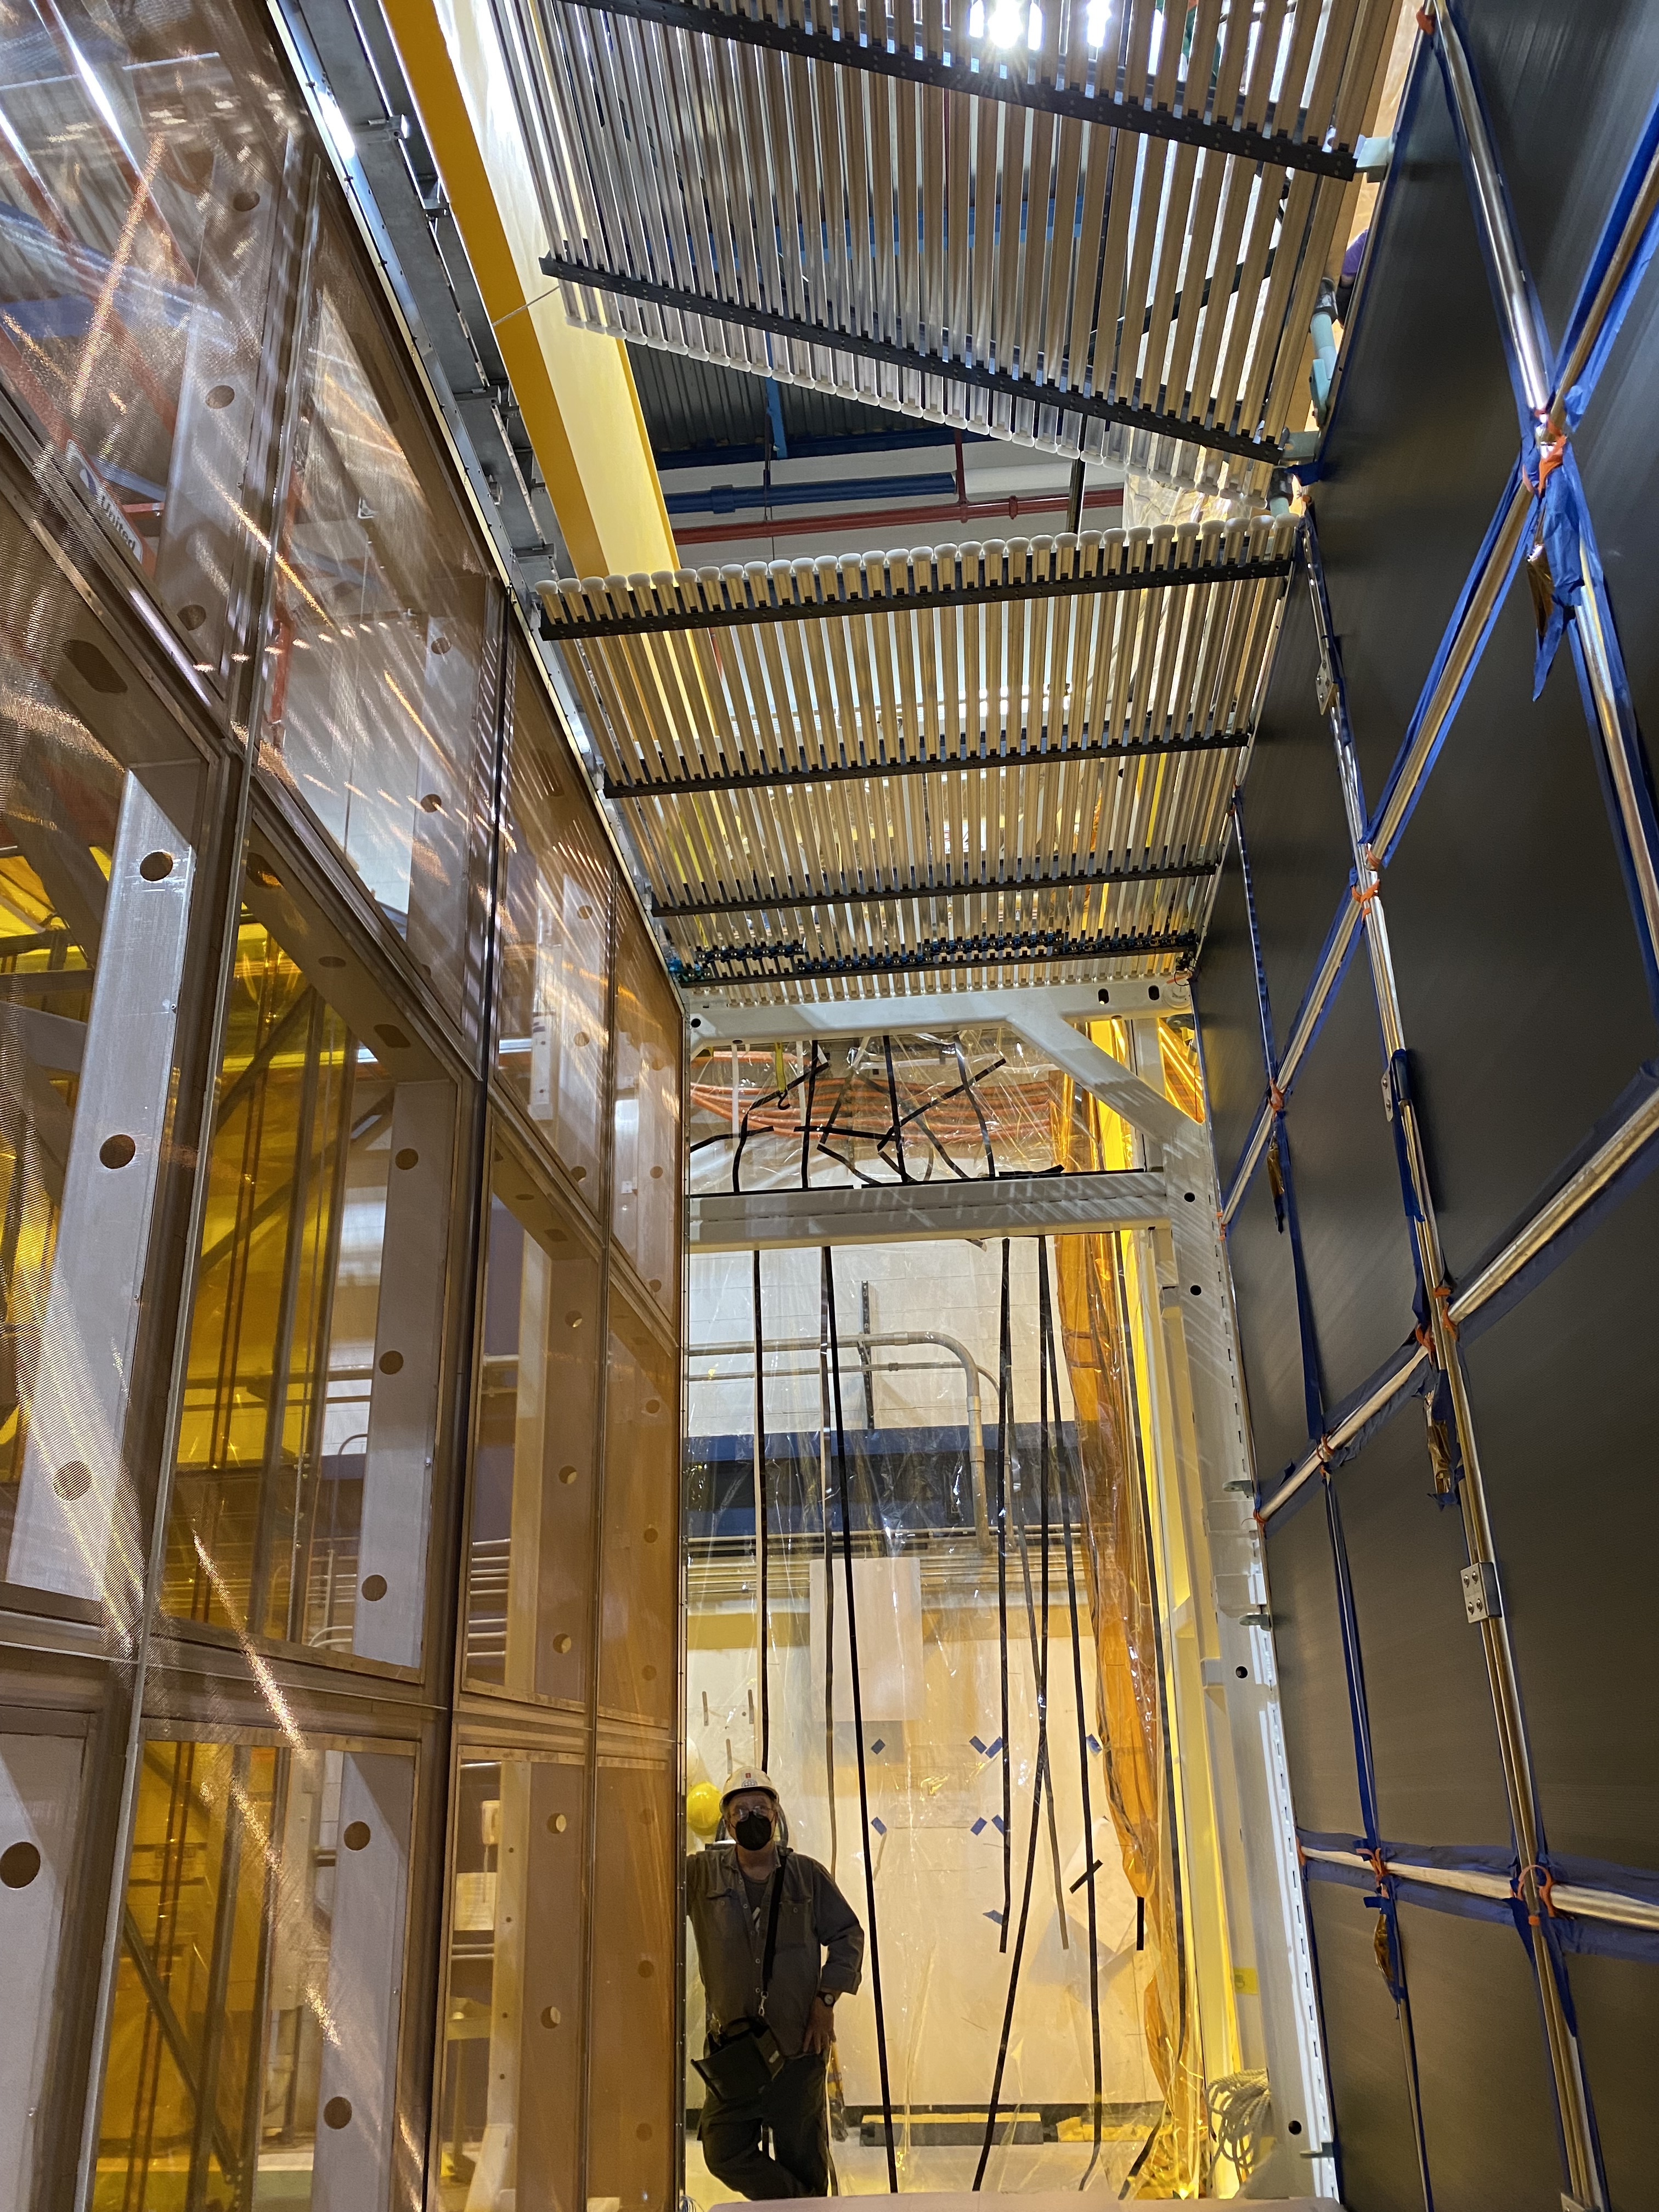
\includegraphics[width=\textwidth]{Figures/field_cage_1.jpeg}
        \caption{}
    \end{subfigure}
    \hfill
    \begin{subfigure}[t]{0.48\textwidth}
        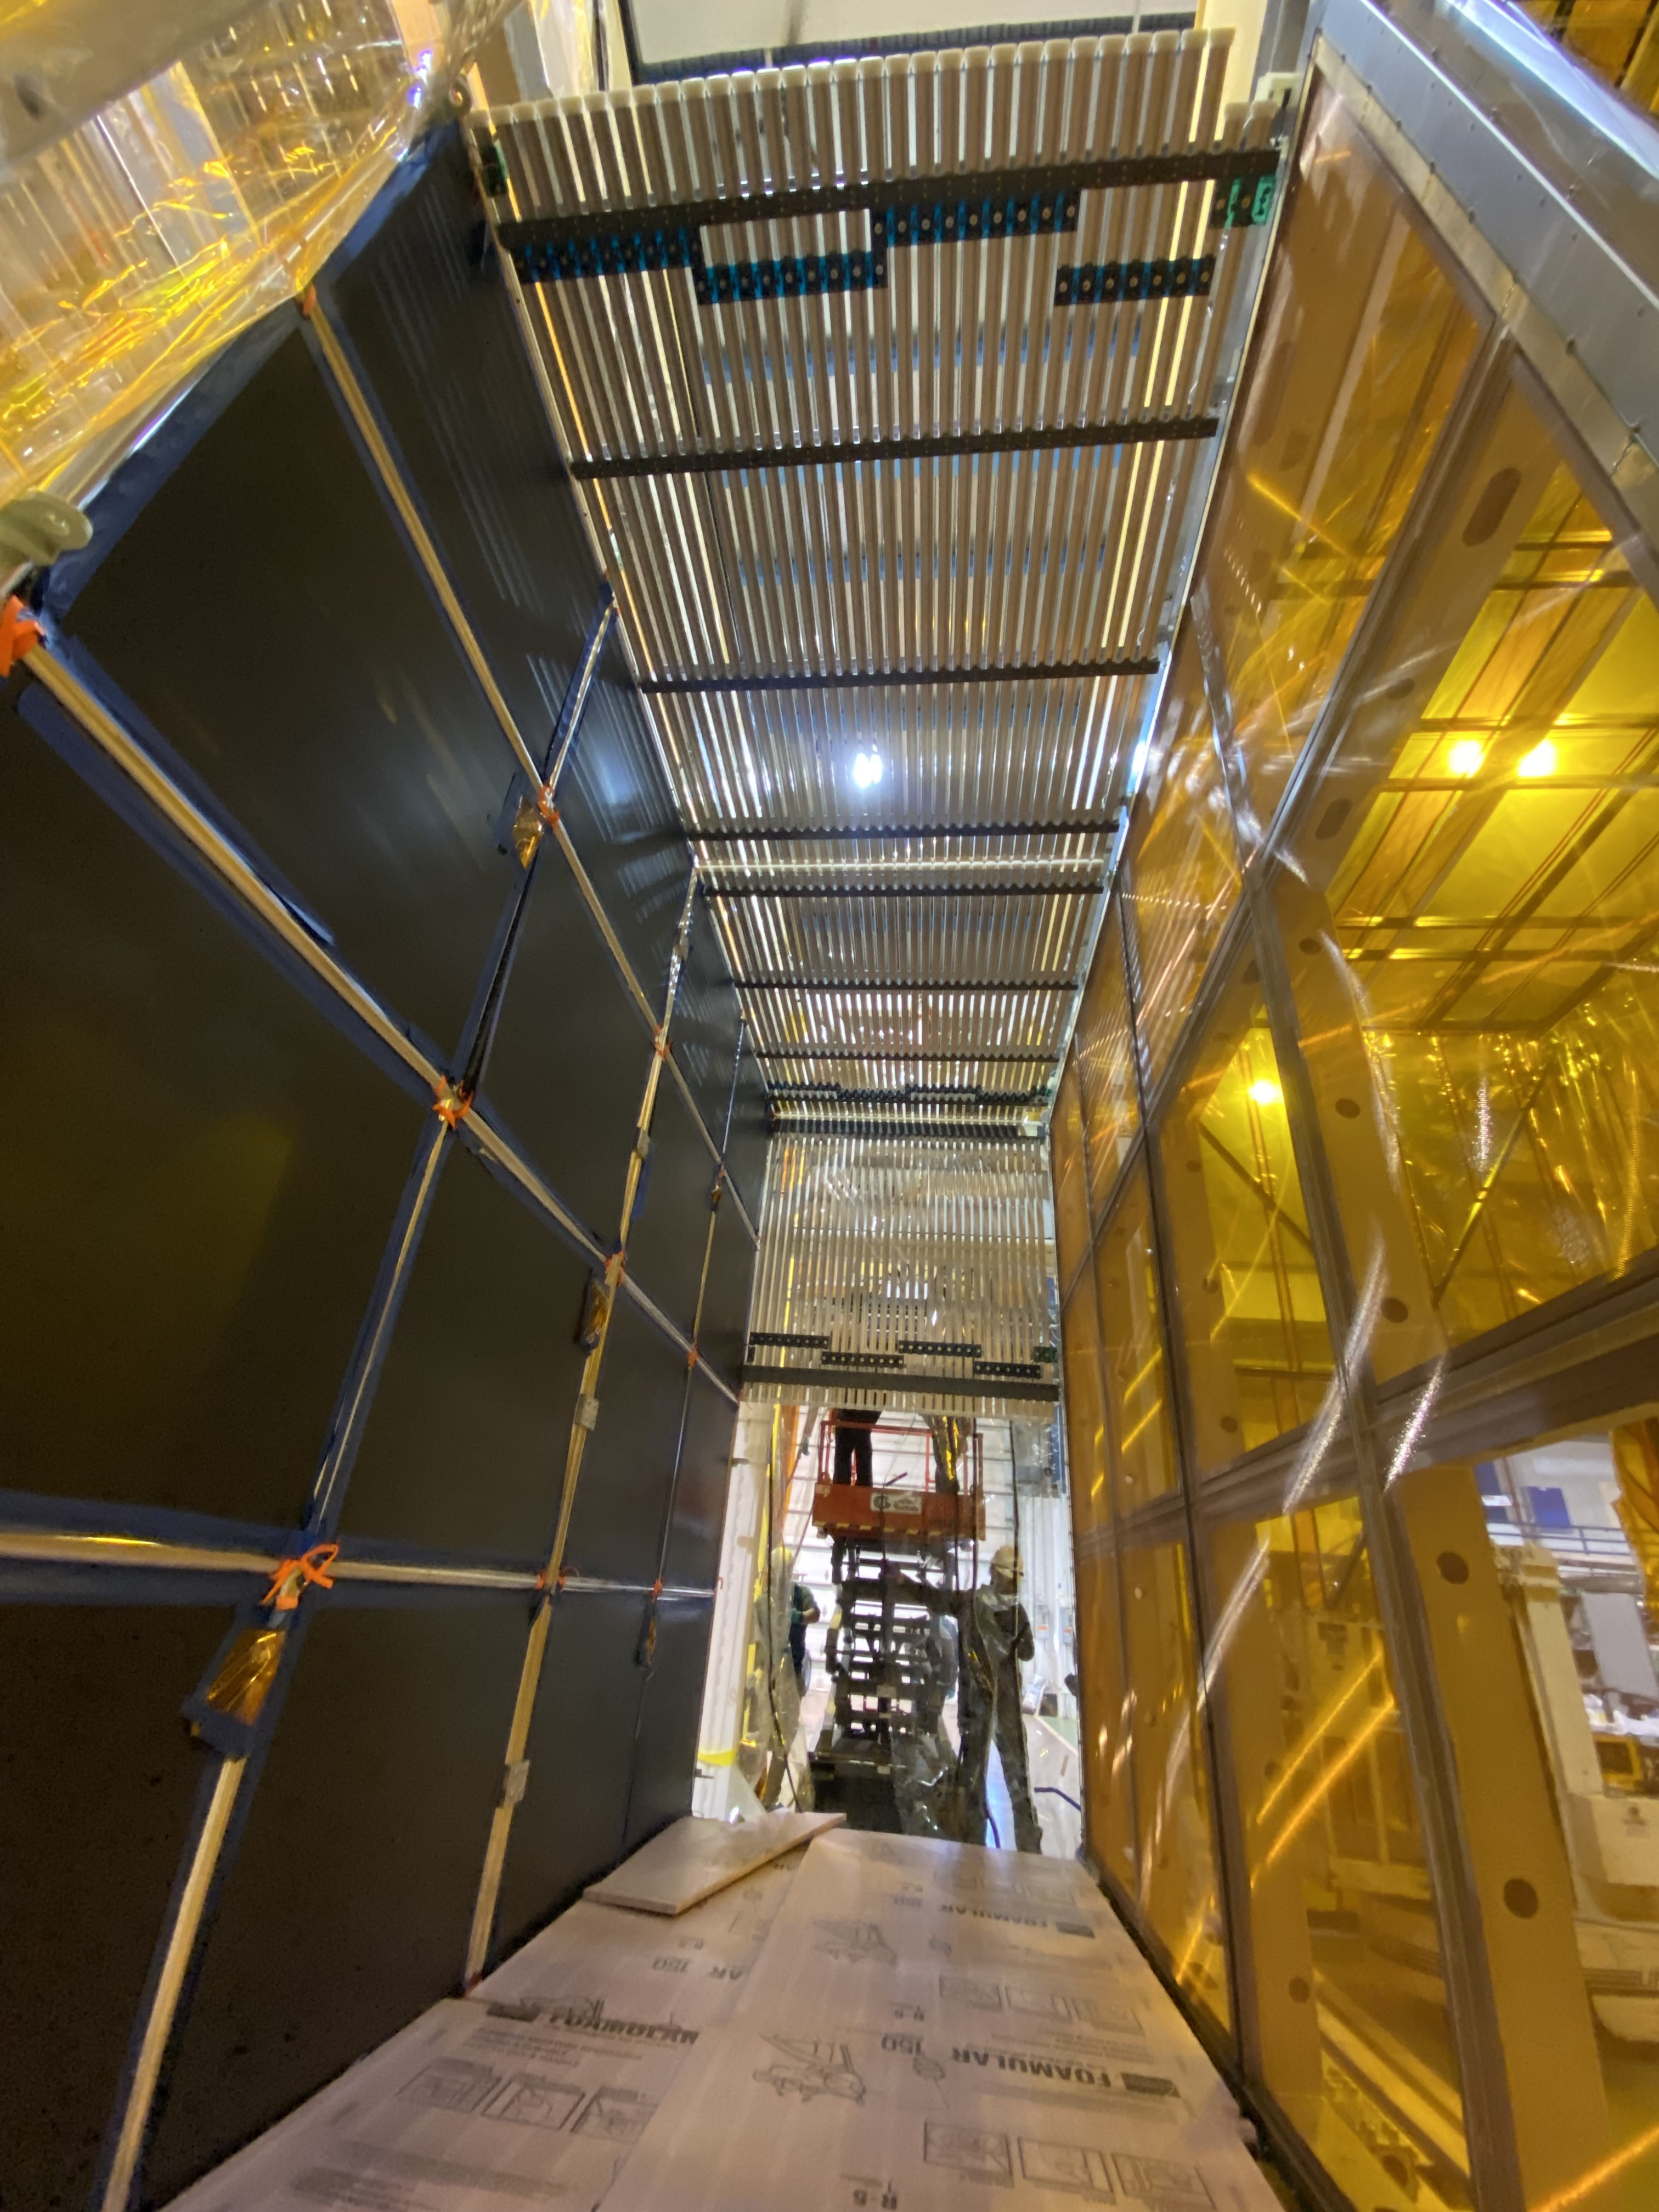
\includegraphics[width=\textwidth]{Figures/field_cage_2.jpeg}
        \caption{}
    \end{subfigure}
	\caption{On the left, a picture one of the top field cage modules being lowered to it place. Next to it, you can see another one already installed. At be back, you can see John Najdzion, the technician responsible for the installation procedures. On the right, you can see a pictur of the East side of the field cage with two top modules installed and one module of the North side installed.}
    \label{field_cage}
\end{figure}
